\chapter{\acs{EsPy} Tutorials}
\label{chap:inserts}
This appendix comprises in insert from a chapter of the \ac{EsPy}
documentation.  The chapter features tutorials describing how to use the
package's \ac{API} for the consideration of \ac{1D} and \ac{2DJ} \ac{NMR}
datasets. These tutorials provide a short description of the key features
associated with the package, and is an ideal initial point of reference for new
users to gain familiarity with \ac{EsPy}.

\newpage
\stepcounter{section}
\phantomsection
\addcontentsline{toc}{section}{\protect\numberline{\thesection}\acs{1D} Tutorial}
\sectionmark{\acs{1D} Tutorial}
\includepdf[%
    pages={13-19},%
    pagecommand={\thispagestyle{fancy}},%
    offset=0 -1cm,%
]{espy-docs.pdf}

\stepcounter{section}
\phantomsection
\addcontentsline{toc}{section}{\protect\numberline{\thesection}\acs{2DJ} Tutorial}
\sectionmark{\acs{2DJ} Tutorial}
\includepdf[%
    pages={20-27},%
    pagecommand={\thispagestyle{fancy}},%
    offset=0 -1cm,%
]{espy-docs.pdf}
